\section{Part 1.2: Parallel Clients with Ray}\label{sec:p12}
\subsection{Actor implementation and required convergence results}
Ray Core Actors are stateful remote objects \citep{rayactors}. Each round creates one Actor for each of four uniformly sampled clients. Actors load their assigned data and run the Part 1.1 local-training routine from the same broadcast. The driver waits for all four updates and aggregates in sampled order, preserving floating-point summation order despite asynchronous completion. A \texttt{finally} block kills the Actors and verifies process exit and CPU-resource return before the next round.

The selected strategy allocates one CPU and zero GPUs per Actor; the alternative benchmark allocates one CPU and 0.25 GPU, sharing one device among four Actors. Both meet the assignment's limits. Actors exist only for selected clients within each round, and all parallelism uses Ray Core directly.

Training uses four clients per round, $E=3$, learning rate 0.3, batch size 32, seed 2026, and 80 rounds (\cref{fig:raycurves}). Final training/validation accuracies are 73.57\%/70.70\%, with losses 0.947290/1.102742. Validation instead selects round 78 at 72.30\%. That checkpoint correctly classifies 2,672/3,621 held-out examples, yielding \textbf{73.79\% test accuracy}.

\begin{figure}[htbp]
\centering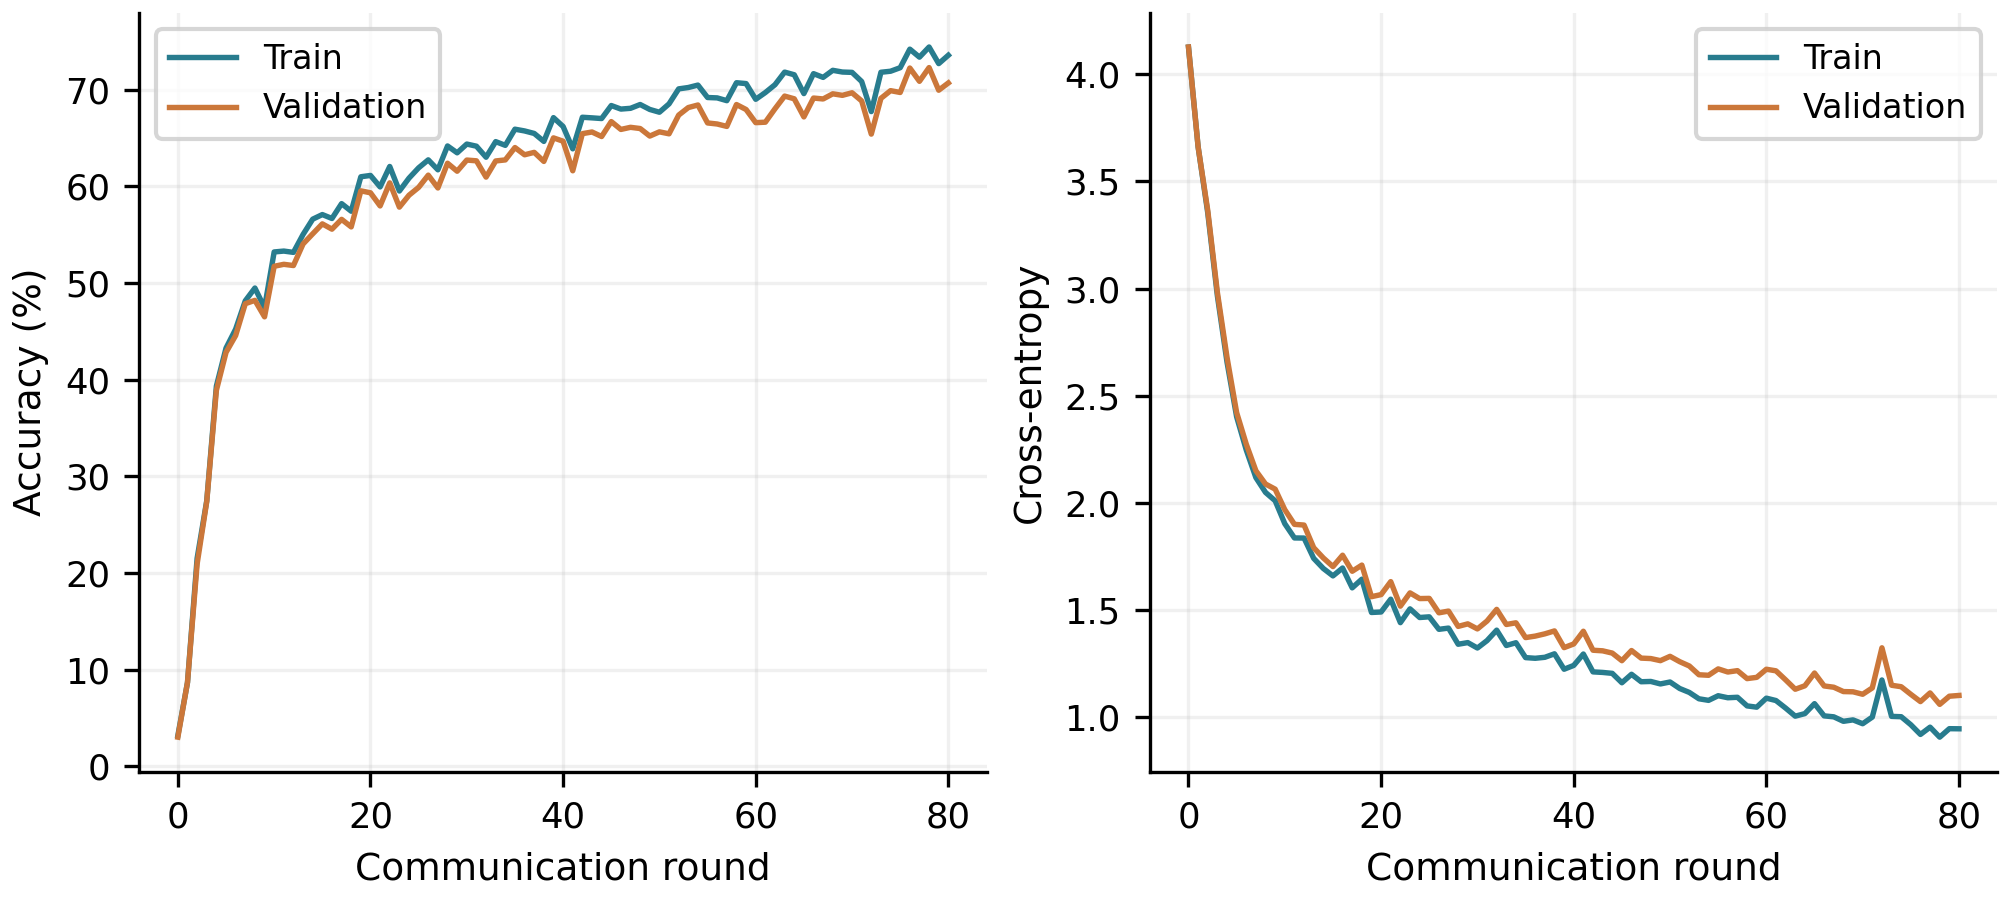
\includegraphics[width=\linewidth]{figures/part1_2/ray_convergence.png}
\caption{Ray training and validation accuracy (left) and cross-entropy (right), including round zero. Four CPU Actors participate per round with $E=3$, learning rate 0.3, and seed 2026. Validation selects round 78.}\label{fig:raycurves}
\end{figure}

\subsection{Scientific Validation and Edge Cases}\label{sec:p12validation}
\subsubsection{A. Numerical correctness of parallel FedAvg}
A matched one-round comparison tests whether parallel execution preserves synchronous FedAvg. Clients 25, 67, 16, and 36 have training sizes 94, 314, 300, and 182. Both implementations use identical initial weights and keyed minibatches at $E=3$ and learning rate 0.3, with an independent weighted-average calculation as an arithmetic reference.

On CPU, every local update, the aggregate, and all training/validation metrics match exactly (maximum difference 0.0; parameter tolerance $10^{-6}$). The independent aggregation error is $1.5521\times10^{-8}$. Fractional-GPU Actors differ from CPU by $2.9802\times10^{-8}$ globally and at most $5.9605\times10^{-8}$ locally, within the $10^{-4}$ cross-device tolerance.

The full 80-round CPU comparison also produces identical selections and metrics, with final parameter difference 0.0 (\cref{fig:raymatch}). Ray therefore preserves the tested serial learning trajectory. The independent Part 1.1 identities address shared-code correctness; the GPU comparison covers only one round.

\subsubsection{B. Actual concurrency, process lifecycle, and memory}
Concurrency was measured from distinct process IDs and training start/finish timestamps, rather than inferred from Actor creation. The intervals begin after the common release barrier. Four training calls overlap in all 80 rounds; every round returns four CPUs and leaves no Actor process alive. \Cref{fig:timeline} illustrates round 1.

\begin{figure}[htbp]
\centering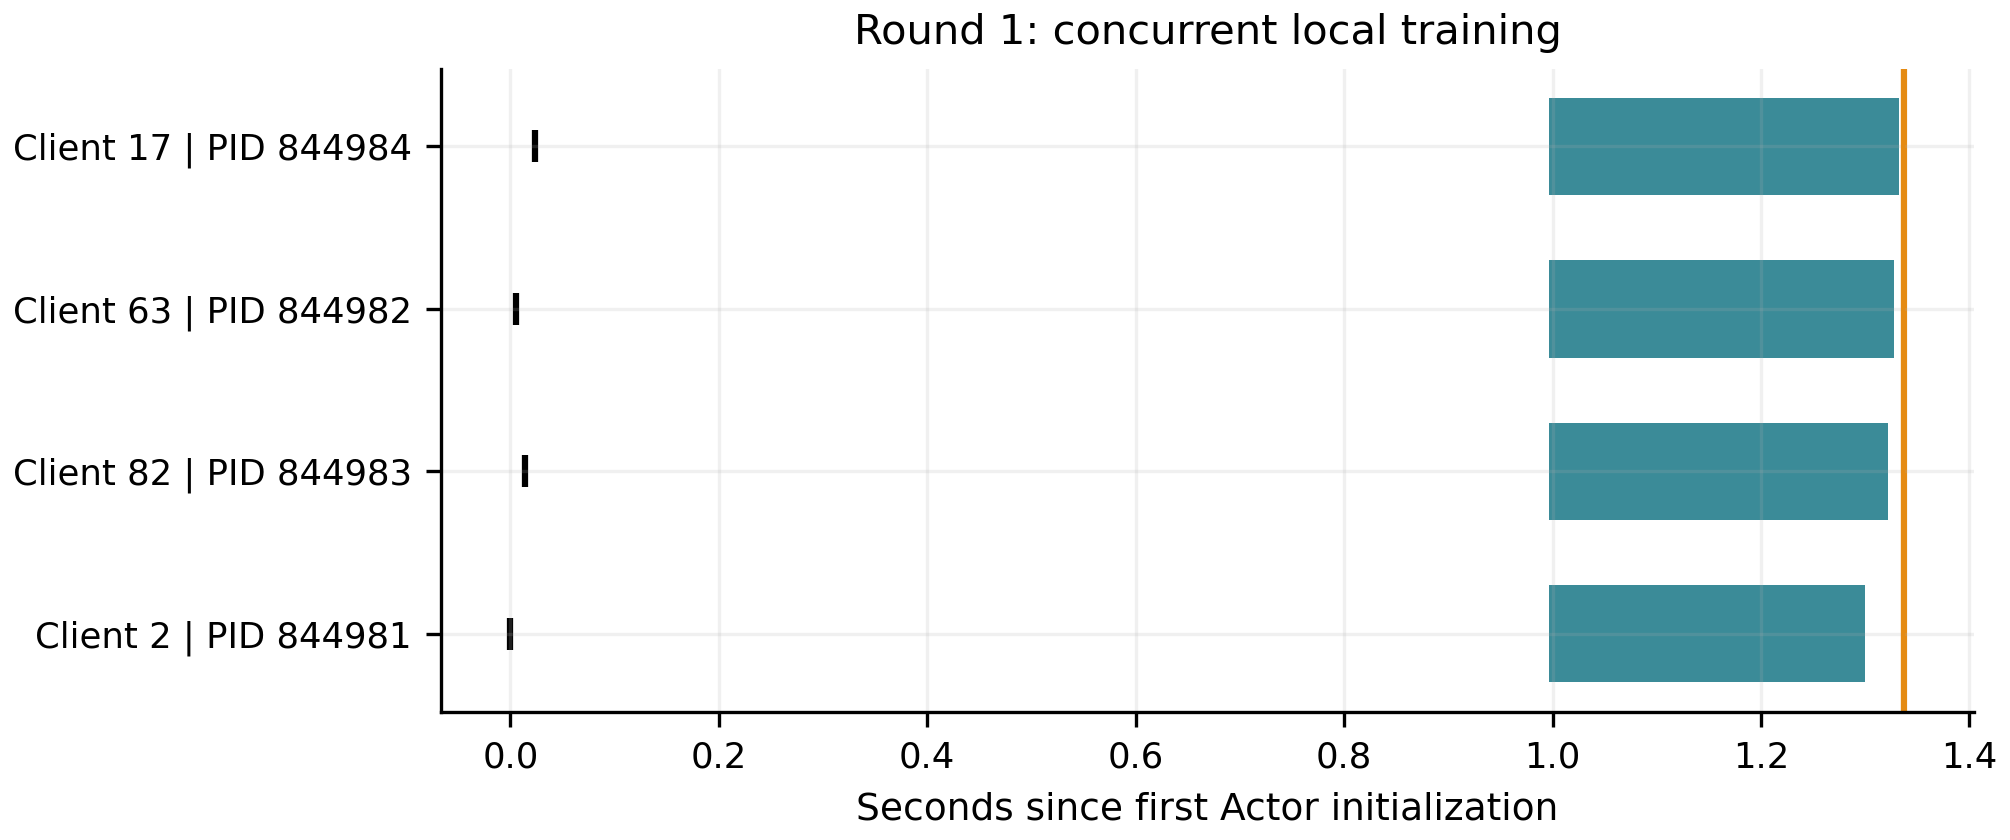
\includegraphics[width=\linewidth]{figures/part1_2/actor_execution_timeline.png}
\caption{Round-1 Actor execution timeline for the CPU run. Black ticks mark initialization, teal intervals local training, and orange aggregation after all updates finish. Four distinct client processes overlap; times are relative to the first Actor initialization.}\label{fig:timeline}
\end{figure}

The mean fastest-to-slowest completion gap is 0.03293 seconds (maximum 0.14037), quantifying one component of synchronous straggler waiting. Driver RSS rises by only 1.43 MiB, from 1,171.49 to 1,172.92 MiB. Together with process exit and resource return, this indicates successful lifecycle cleanup over the run.

\subsubsection{C. Efficiency: concurrent execution is slower here}
Concurrency does not guarantee speedup: savings in local computation must exceed lifecycle and coordination costs. Three repeats of the same four-client round compare one-thread sequential CPU, four one-thread CPU Actors, and four fractional-GPU Actors. Every repeat creates fresh Actors. Among numerically valid strategies, the lower median complete round time selects CPU; \cref{tab:raytiming} reports means and sample SDs.

\begin{table}[htbp]
\centering
\caption{Measured strategy benchmark and full-workload timings. Three-repeat round timers include the Actor lifecycle and release barrier, but exclude global evaluation/checkpointing. Runtime initialization is measured separately and added once.}\label{tab:raytiming}
\begin{tabularx}{\linewidth}{Yrrr}
\toprule
Strategy & Round mean $\pm$ SD (s) & Ray init. (s) & Three rounds + init. (s)\\
\midrule
Sequential CPU & $0.03342\pm0.00173$ & 0 & 0.10027\\
Ray CPU & $3.00794\pm0.41718$ & 5.11084 & 14.13466\\
Ray shared GPU & $4.11489\pm0.69292$ & 3.34036 & 15.68502\\
\midrule
\multicolumn{4}{l}{Full 80-round workload: sequential CPU 11.94713 s; Ray CPU 276.13739 s.}\\
\bottomrule
\end{tabularx}
\end{table}

The full Ray workload takes 272.81936 seconds plus 3.31802 seconds for runtime initialization, totaling 276.13739 seconds, versus 11.94713 seconds sequentially. Both include model initialization, round-zero and later evaluation, and checkpoint/history I/O; Ray also includes cleanup and shutdown. Python launch and prior data preparation are excluded. Thus
\begin{equation}
\text{speedup}=\frac{11.94713}{276.13739}=0.04326,
\qquad\text{slowdown}=23.11.\label{eq:speedup}
\end{equation}
These full-workload times differ from the isolated round benchmark, which excludes global evaluation and checkpoint I/O. Runtime initialization is added once in each comparison.

\begin{figure}[htbp]
\centering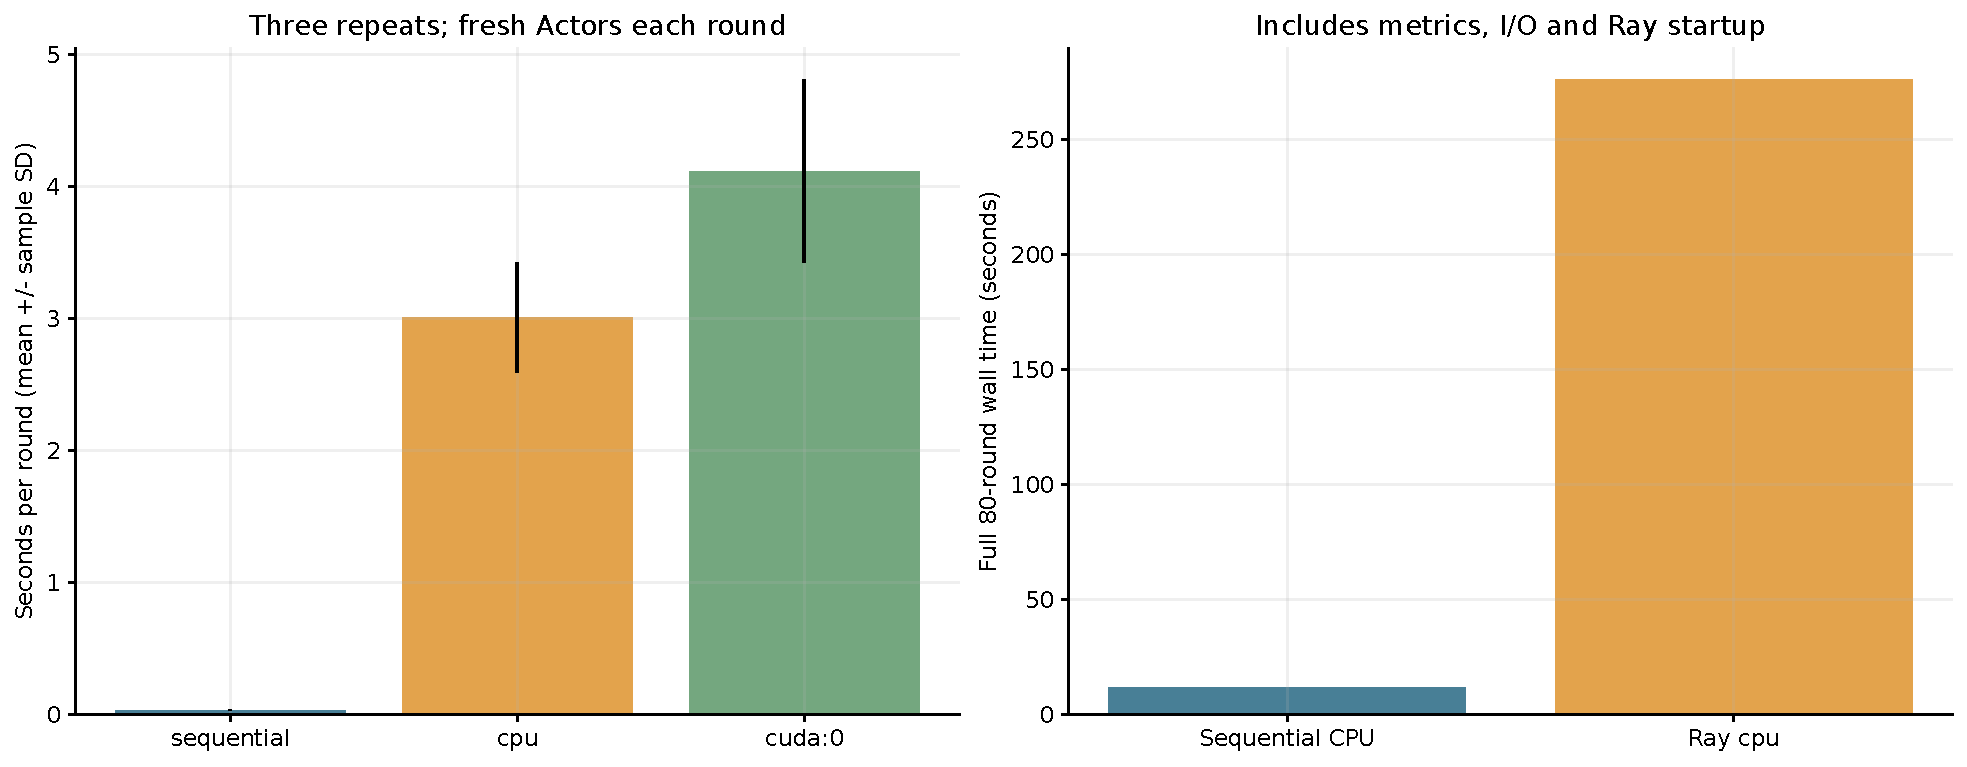
\includegraphics[width=\linewidth]{figures/part1_2/parallel_performance.pdf}
\caption{Complete round time (left; mean and sample SD over three repeats with fresh Actors) and full 80-round workload time (right; including evaluation, I/O, and Ray initialization once).}\label{fig:rayperformance}
\end{figure}

Mean Actor startup is 2.68811 seconds, versus 0.31683 seconds per local training interval; cleanup and aggregation average 0.09368 and 0.00117 seconds. Startup therefore dominates this small 108,478-parameter workload. The 0.15-second common release delay is also included in round time. Imports, model construction, serialization, and scheduling contribute overhead; GPU Actors additionally incur context and transfer costs. The timers do not isolate every component, but clearly explain the measured slowdown (\cref{fig:rayperformance}).

\subsubsection{Failures, unavailable resources, and deterministic recovery}
\begin{table}[htbp]
\centering
\caption{Ray failure injection and edge cases. Allocation failures and unavailable GPUs are controlled injections or logical resource shortages.}\label{tab:rayedges}
\begin{tabularx}{\linewidth}{p{0.24\linewidth}YY}
\toprule
Case & Experiment and expected response & Recorded result\\
\midrule
Actor exception & One of four Actors raises a runtime error; reject the round and clean up. & Explicit Ray task error; four CPUs returned.\\
Allocation failure & Inject \texttt{MemoryError}, without exhausting physical RAM. & Explicit error; four CPUs returned.\\
Non-finite update & Fill one returned parameter with NaN. & Aggregator raises \texttt{FloatingPointError}; no valid aggregate.\\
Unavailable GPU & Request fractional GPUs in a CPU-only runtime with a 0.5 s deadline. & \texttt{GetTimeoutError}; four CPUs returned.\\
Interrupted round & Inject interruption before aggregation/commit, then replay. & Explicit interruption; replay parameter difference 0.0.\\
Tiny / missing classes & Synthetic sizes 1, 2, 7, 13, all class zero; compare serial/Ray. & Maximum parameter difference 0.0.\\
Unequal sizes & Real counts 94, 314, 300, 182; count-weighted reference. & CPU manual aggregation error $1.55\times10^{-8}$.\\
Sampling & 10,000 rounds, four unique clients, same/different seed checks. & Counts 351--439 versus mean 400; maximum $|z|=2.501$.\\
\bottomrule
\end{tabularx}
\end{table}

Failure tests in \cref{tab:rayedges} verify that incomplete rounds never contribute partial averages. Automatic Actor retries are disabled; deterministic replay starts from the last committed checkpoint and leaves the broadcast unchanged. The resource failures are controlled injections or logical shortages, not actual RAM exhaustion or hardware outages.



